% !TeX root = ../main.tex
% Add the above to each chapter to make compiling the PDF easier in some editors.

\chapter{Introduction}\label{chapter:introduction}

% % Cloud computing is the on-demand consumption of compute power, storage, database, applications, and any IT resources through the Internet following pay-as-you-go pricing model. 
% % The most basic way to define what the ‘Cloud’ is that it is a computer located somewhere else that is accessed via the Internet and utilized in some way. 
% % Web services is also another name for what people call the cloud. 
% % The cloud is comprised of server computers located in different locations around the world. 
% % When we use a cloud service like Amazon Web Services (AWS) or Google Cloud Architecture or Microsoft Azure, we are actually utilizing the computers belonging to these Cloud Service Providers [CSPs].

% % The principle of cloud computing is remaining as it is, but, the need for shared working principle, enhancements in fast response of the services, agility of resource provisioning, and minimized management hurdles has been the targets of hyper scale CSPs. 
% % Inspecting the level of capital investment and management involved to reach the above objectives, there are many researches proposed several reference models. 
% % Hyper scale data centers will grow from 338 in number at the end of 2016 to 628 by 2021. 
% % They will represent 53 percent of all installed data center servers by 2021. 
% % This kind of drastic increase in the computational requirements, there is a need for transforming the ‘traditional data centers’ into ‘hyper scale datacenters’ sophisticated with high levels of abstraction and virtualization. 
% % Recent technical advancement in the virtualization technologies which are very promising to achieve hyper scale data centres easily.

% % In the initial stages virtualization used as the mean for software and service consolidation by which attained the maximum utilization of the resources and easy management. 
% % During the initial phase, there was a common sharing of hardware. 
% % In the next phase, there was a pool of Virtual Machines (VMs) created on a server and each VM carry a copy of an operating system. 
% % Later, it advanced into the concept of containers where it included, OS level virtualization. 
% % The containers are the platform sufficient enough to hold the resources needed for running a specific application. 
% % It achieved higher abstraction of resources comparing with VMs. 
% % In containerization, resource provisioning is much faster than VMs.

% % Apart from the efficiencies and faster rate of provisioning of resources through containerization, further enhancements are constrained with the basic infrastructural elements called servers. 
% % Serverless computing is a model of pooling and utilizing the resources which includes OS, runtime environments and hardware.

Cloud computing as defined by the cloud providers is an on-demand delivery of Information Technology (IT) resources like compute power, storage, database, applications over the Internet with pay-as-you-go pricing. 
% These IT resources reduced the computation time and ideal resource cost, wherein increasing the demand of network bandwidth for communication, 
% But in a swift speed cloud computing took over the field of Data Science and Internet of Things services.
% In the initial stages, multiple users were allowed to use the same hardware with different permissions in order to make an efficient use of resources. 
Function as a Service (Faas) is a serverless backend cloud computing platform provided by the cloud providers. 
This platform allows the users to develope, run and manage multiple lightweight functions constituting an application without worrying about preparing the runtime, managing deployment and infrastructure related concerns.
Thus in FaaS, the responsibilities of the cloud service provider include the management of the datacenter, server and the runtime environment.
In contradiction to other cloud models, the more responsibility is vested on the shoulder of Cloud Service Provider (CSP) and the developer is relieved from the management and maintenance complications any further.
Since the responsibility of management and maintenance is vested in the shoulder of CSP, the response time of every function partially relies on both the developer and the CSP.

Response time is the total amount of time a function or a service takes to respond to a request. 
Response time depends on the network delay and function execution delay.
Function execution depends on the memory and Central Processing Uint (CPU) power availability.
Utilization of CPU power and memory can be spiked by different aspects like deploying multiple functions in the same node and continuously increasing the event load of a particular function.
These aspects influence the response time to a function request, thus resulting in the significant drop of the quality of the service provided by the FaaS platform.

% Serverless computing or Function-as-a-Service (FaaS) is defined as a software architecture where an application is decomposed into ‘triggers’ (events) and ‘actions’ (functions), and there is a platform that provides a seamless hosting and execution environment. 
% The application developer’s concern only for light weighted and stateless functions that can be executed through an API based on the on-demand principle. 
% The application consumes the resources to the point of execution and later the resources are released. 
% The price model includes only the amount of time in which the resources were in use and the application developer need not to pay for resources until they are executed, thus it is referred to as ‘serverless’.

% In serverless computing, the responsibilities of the cloud service provider include the management of the datacenter, server and the runtime environment. 
% A contrast to the other cloud models, the more responsibility is vested on the shoulder of cloud service provider and the developer is relieved with the management and maintenance complications any further.\cite{rajan2018serverless}

% Cold start refers to the state our function was when serving a particular invocation request. 
% A serverless function is served by one or multiple micro-containers. 
% When a request comes in, our function will check whether there is a container already running to serve the invocation. 
% When an idle container is already available, we call it a “warm” container. 
% If there isn’t a container readily available, the function will spin up a new one and this is what we call a “cold start”.

% When a function in a cold state is invoked, the request will take additional time to be completed, because there’s a latency in starting up of a new container. 
% That’s the problem with cold starts: they make our application respond slower. 
% In the “instant-age” of the 21st century, this could be a big problem.

% The state of the art solution for the cold start problem is keeping functions warm.
% But we hope decreased transparency is the actual problem for the cold start problem.
% Therefore in this report, we are trying to predict the response time of a function by analyzing different metrics and overcome the cold start problem by predicting the number of containers required for a function in a particular time.  

% \subsubsection{Types of Metrics:}

% \begin{enumerate}
%     \item User Centric
%     \item FaaS Platform Centric
%     \item IaaS Platform Centric
% \end{enumerate}

% \begin{table}[htpb]
%     \caption[Metrics table]{Types of Metrics}\label{tab:sample}
%     \centering
%     \begin{tabular}{l l l}
%       \toprule
%         User Centric & FaaS Platform Centric & IaaS Platform Centric \\
%       \midrule
%         Cost, & Number of Functions, & Number of Core,\\
%         Response time, & Number of Containers, & Number of Virtual Machines,\\
%         Number of Requests/ & Number of Invocations & Memory used,\\
%         Workload & Execution time (Cold start/ & Storage used \\
%         & Warm start & \\
%         & + Response time) & \\ 
%       \bottomrule
%     \end{tabular}
%   \end{table}


\section{Problem:}

The increasing response time for function requests causes a significant drop in the quality of service. 
The plan of this proposal is to define a stable response time by defining a model which is capable of stating the required resources to acquire a stable response time.
The figure below states the increase in request per minute increases the cpu rate and memory utilization which inturn defines the constant increase in response time.

\begin{figure}[htpb]
  \centering
  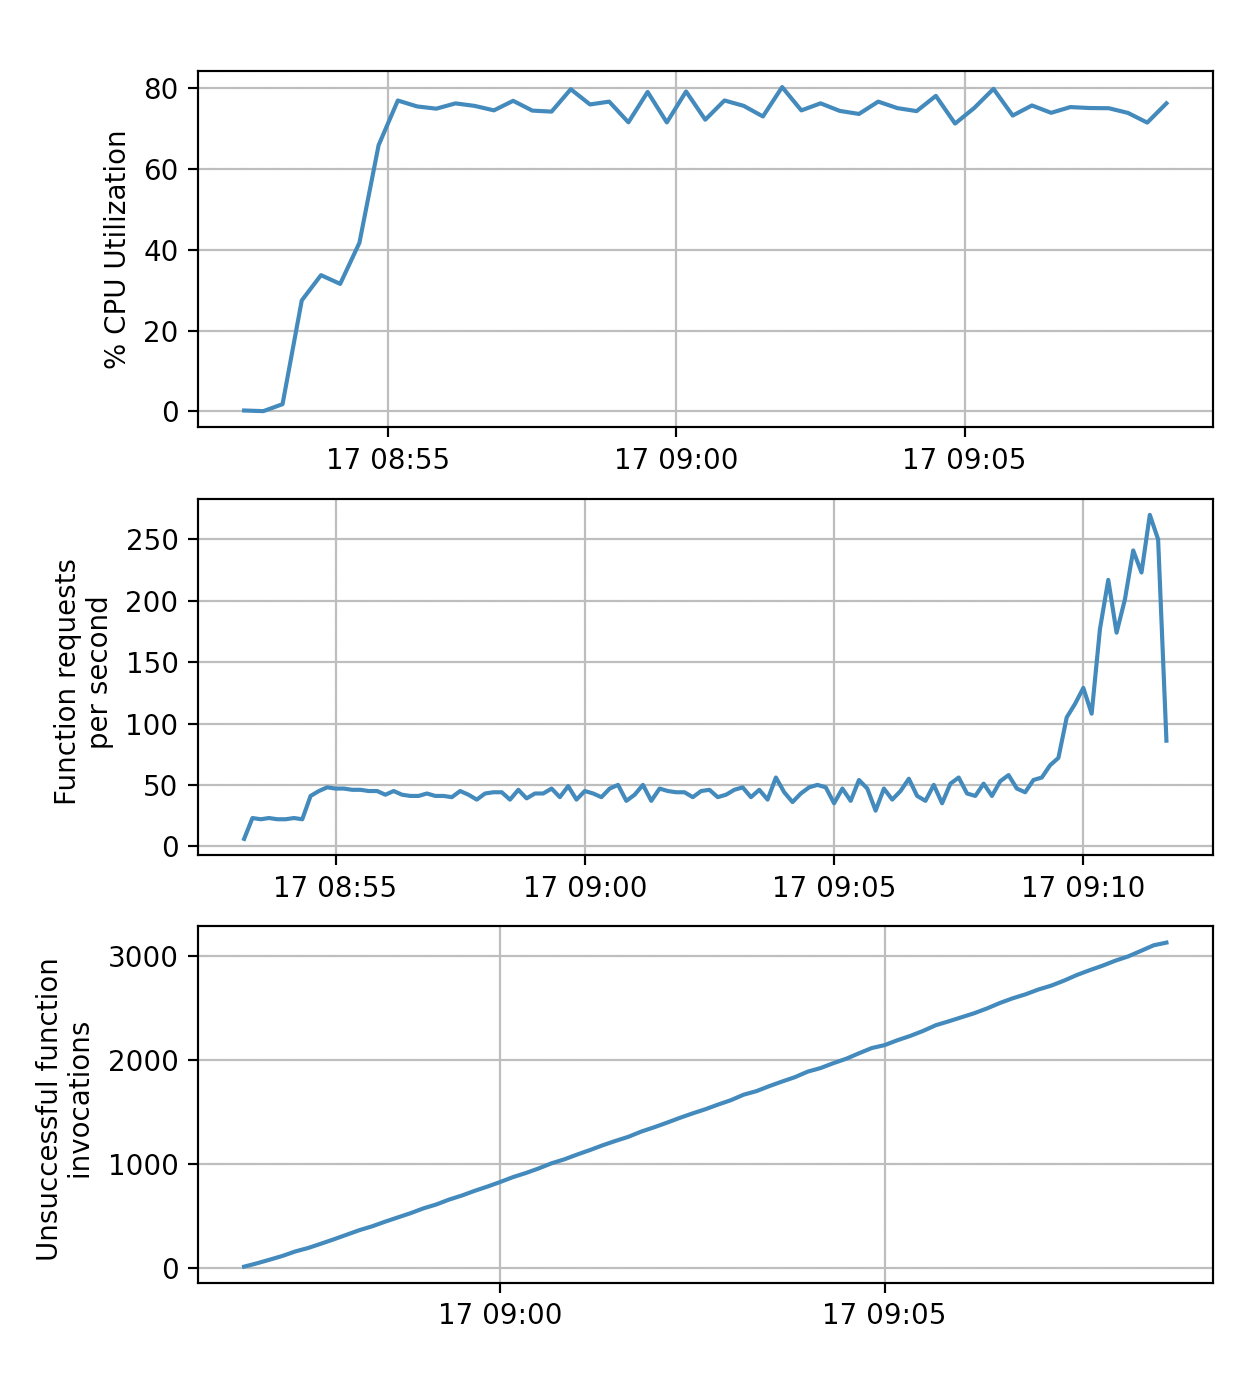
\includegraphics[width=1\textwidth]{figures/graph2}
  \caption{CPU Rate increases with the increase in number of requests} \label{fig:tumslide}
\end{figure}

\begin{figure}[htpb]
  \centering
  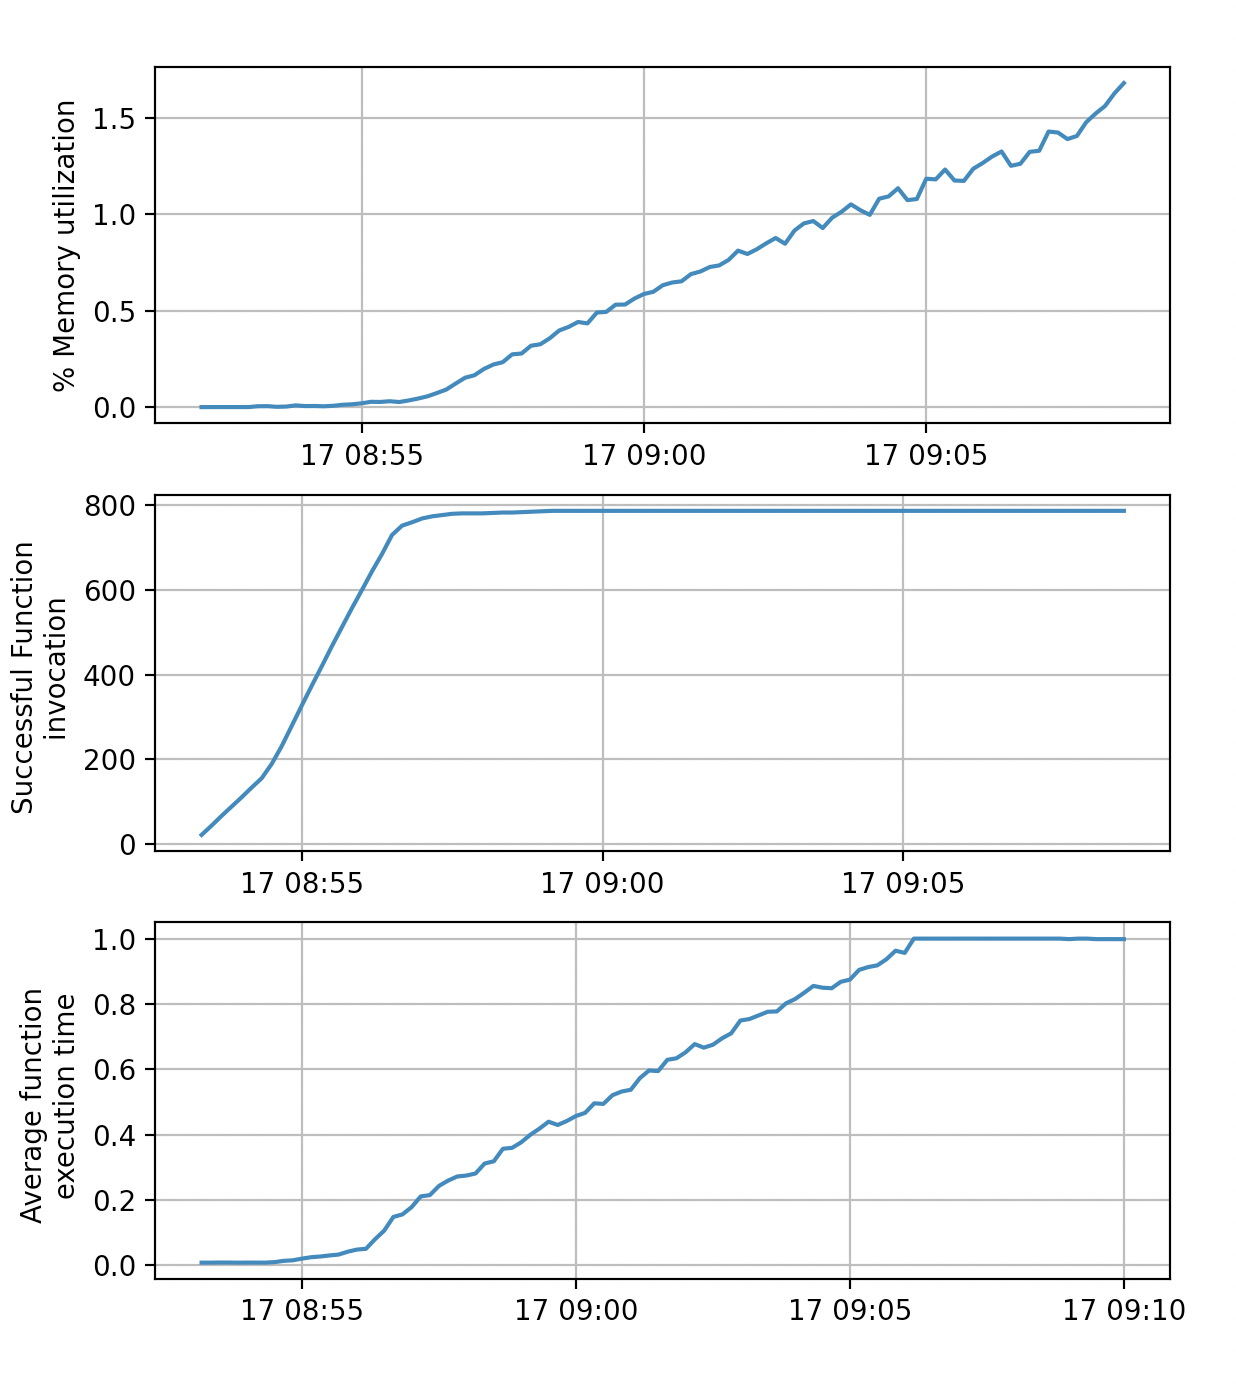
\includegraphics[width=1\textwidth]{figures/graph1}
  \caption{Response time increases with the increase in memory utilization and CPU rate} \label{fig:tumslide}
\end{figure}

\section{Objective:}

The plan of this proposal is to define a model, that can predict the resources required for a particular response time. 
Using the metrics below,

\subsubsection{Types of Metrics:}

\begin{enumerate}
    \item User Centric
    \item FaaS Platform Centric
    \item IaaS Platform Centric
\end{enumerate}

\begin{table}[htpb]
    \caption[Metrics table]{Types of Metrics}\label{tab:sample}
    \centering
    \begin{tabular}{l l l}
      \toprule
        User Centric & FaaS Platform Centric & IaaS Platform Centric \\
      \midrule
        Cost, & Number of Functions, & Number of Core,\\
        Response time, & Number of Containers, & Number of Virtual Machines,\\
        Number of Requests/ & Number of Invocations & Memory used,\\
        Workload & Execution time (Cold start/ & Storage used \\
        & Warm start & \\
        & + Response time) & \\ 
      \bottomrule
    \end{tabular}
  \end{table}

\section{Outline:}

\subsubsection{Sample data table:}
\begin{table}[htpb]
  \caption[Data table]{Data Metrics}\label{tab:sample}
    \begin{tabular}{lllllll}
    Time               & CPU Rate              & Mem Utiliz    & HttpReq & res200 & res502 & resTime              \\
    2020-05-17 08:52:10 & 0.12                & 0.00029 & 38.0      & 21.0        & 17.0        & 0.0078         \\
    2020-05-17 08:52:20 & 0.26                & 0.00058 & 92.0     & 43.0        & 49.0        & 0.0077 \\
    2020-05-17 08:52:30 & 0.28                & 0.00058 & 150.0     & 66.0        & 84.0        & 0.0082 \\
    2020-05-17 08:52:40 & 0.29 & 0.00059 & 208.0     & 88.0        & 120.0       & 0.0080 \\
    2020-05-17 08:52:50 & 0.31                & 0.00060 & 273.0     & 110.0       & 163.0       & 0.0077 \\
    2020-05-17 09:03:00 & 1645.40  & 0.96464    & 3600.0     & 787.0       & 2813.0      & 0.8150   \\
    2020-05-17 09:03:10 & 1674.07  & 0.92836    & 3646.0     & 787.0       & 2859.0      & 0.8344   \\
    2020-05-17 09:03:20 & 1706.42  & 0.98191    & 3689.0     & 787.0       & 2902.0      & 0.8551   \\
    2020-05-17 09:03:30 & 1735.42             & 1.01262     & 3737.0     & 787.0       & 2950.0      & 0.8497         \\
    2020-05-17 09:03:40 & 1765.65  & 1.05117     & 3778.0     & 787.0       & 2991.0      & 0.8479   \\
    2020-05-17 09:03:50 & 1795.48             & 1.02082    & 3831.0     & 787.0       & 3044.0      & 0.8678   \\
    2020-05-17 09:04:00 & 1825.44             & 0.99666    & 3885.0     & 787.0       & 3098.0      & 0.8744   \\
    2020-05-17 09:04:10 & 1854.94  & 1.08041    & 3911.0     & 787.0       & 3124.0      & 0.9041  
    \end{tabular}
\end{table}


%   Data like this are collected and used to create a model that can predict the resource requirements for a particular response time.






























% Use with pdfLaTeX and Biber.

% \section{Section}
% Citation test (with Biber)~\parencite{latex}.

% \subsection{Subsection}

% See~\autoref{tab:sample}, \autoref{fig:sample-drawing}, \autoref{fig:sample-plot}, \autoref{fig:sample-listing}, \autoref{fig:tum}, \autoref{fig:tumslide}.

% \begin{table}[htpb]
%   \caption[Example table]{An example for a simple table.}\label{tab:sample}
%   \centering
%   \begin{tabular}{l l l l}
%     \toprule
%       A & B & C & D \\
%     \midrule
%       1 & 2 & 1 & 2 \\
%       2 & 3 & 2 & 3 \\
%     \bottomrule
%   \end{tabular}
% \end{table}

% \begin{figure}[htpb]
%   \centering
%   % This should probably go into a file in figures/
%   \begin{tikzpicture}[node distance=3cm]
%     \node (R0) {$R_1$};
%     \node (R1) [right of=R0] {$R_2$};
%     \node (R2) [below of=R1] {$R_4$};
%     \node (R3) [below of=R0] {$R_3$};
%     \node (R4) [right of=R1] {$R_5$};

%     \path[every node]
%       (R0) edge (R1)
%       (R0) edge (R3)
%       (R3) edge (R2)
%       (R2) edge (R1)
%       (R1) edge (R4);
%   \end{tikzpicture}
%   \caption[Example drawing]{An example for a simple drawing.}\label{fig:sample-drawing}
% \end{figure}

% \begin{figure}[htpb]
%   \centering

%   \pgfplotstableset{col sep=&, row sep=\\}
%   % This should probably go into a file in data/
%   \pgfplotstableread{
%     a & b    \\
%     1 & 1000 \\
%     2 & 1500 \\
%     3 & 1600 \\
%   }\exampleA
%   \pgfplotstableread{
%     a & b    \\
%     1 & 1200 \\
%     2 & 800 \\
%     3 & 1400 \\
%   }\exampleB
%   % This should probably go into a file in figures/
%   \begin{tikzpicture}
%     \begin{axis}[
%         ymin=0,
%         legend style={legend pos=south east},
%         grid,
%         thick,
%         ylabel=Y,
%         xlabel=X
%       ]
%       \addplot table[x=a, y=b]{\exampleA};
%       \addlegendentry{Example A};
%       \addplot table[x=a, y=b]{\exampleB};
%       \addlegendentry{Example B};
%     \end{axis}
%   \end{tikzpicture}
%   \caption[Example plot]{An example for a simple plot.}\label{fig:sample-plot}
% \end{figure}

% \begin{figure}[htpb]
%   \centering
%   \begin{tabular}{c}
%   \begin{lstlisting}[language=SQL]
%     SELECT * FROM tbl WHERE tbl.str = "str"
%   \end{lstlisting}
%   \end{tabular}
%   \caption[Example listing]{An example for a source code listing.}\label{fig:sample-listing}
% \end{figure}

% \begin{figure}[htpb]
%   \centering
%   \includegraphics[width=0.8\textwidth]{tum}
%   \caption[Something else can be written here for listing this, otherwise the caption will be written!]{Includegraphics searches for the filename without extension first in logos, then in figures.} \label{fig:tum}
% \end{figure}

% \begin{figure}[htpb]
%   \centering
%   \includegraphics[width=0.8\textwidth]{figures/tum}
%   \caption{For pictures with the same name, the direct folder needs to be chosen.} \label{fig:tumslide}
% \end{figure}

% \begin{figure}[!tbp]
%   \centering
%   \subfloat[TUM Logo][The logo.]{\includegraphics[height=0.2\textheight]{tum}\label{fig:tum1}}
%   \hfill
%   \subfloat[TUM Slide][The famous slide.]{\includegraphics[height=0.2\textheight]{figures/tum}\label{fig:tum2}}
%   \caption{Two TUM pictures side by side.}
%   \label{fig:sidebyside}
% \end{figure}

% This is how the glossary will be used.

% \Glspl{ddye}, \gls{r0}, \gls{R0}, and \gls{kdeac}. Also, the \glspl{tum} has many \glspl{computer}, not only one \Gls{computer}. Subsequent acronym usage will only print the short version of \glspl{tuma} (take care of plural, if needed!), like here with \gls{tuma}, too. It can also be --> \glsdisp{tum}{hidden}\footnote{Example for a hidden TUM glossary entry.} <--.

% \todo{Now it is your turn to write your thesis.

% This will be a few tough weeks.}

% \done{Nevertheless, celebrate it when it is done!}
